\chapter{Cammini minimi}

{Solitamente si sottintende l'utilizzo su grafi orientati, in caso di grafi non orientati, ogni arco può essere sostituito da una coppia di archi inversamente orientati.}

$G=(V,E,w)$ orientato, $w:E\rightarrow \mathbb{R}$

Un cammino $p$ è una sequenza $<x_0,x_1,\ldots,x_q>$, $\forall i, i\leq i \leq q, (x_{i-1},x_i) \in E$.

$w(p)=\sum_{i=1}^{q} w(x_{i-1},x_i)$ è la funzione ``peso'' di un cammino $p$.

{La distanza $\delta(u,v)$ tra due vertici $u,v \in V$ è definita nel seguente modo:}

{$\delta(u,v) = +\infty$ se non esiste un cammino orientato da u a v}

{$\delta(u,v)=min(w(p))$ minimo dei pesi dove $p$ è il cammino tra $u$ e $v$}

\paragraph{Varianti}

{Esistono quattro diverse varianti di ricerca dei cammini minimi, combinazioni dei due casi di numerosità dei vertici di partenza e di destinazione.}

\begin{table}[]
\centering
\begin{tabular}{ll|l|l|}
\cline{3-4}
                                                 &                               & \multicolumn{2}{c|}{Destinazione}                            \\ \cline{3-4}
                                                 &                               & \multicolumn{1}{c|}{Singola} & \multicolumn{1}{c|}{Multipla} \\ \hline
\multicolumn{1}{|c|}{}                           & \multicolumn{1}{c|}{Singola}
& \specialcell{In: $G(V;E;w)\,u,v\in V$\\Out: $\delta(u,v)$ }
& \cellcolor[HTML]{F8A102}\specialcell{In: $G(V;E;w)\,s\in V$\\Out: $\forall v \in V, \delta(s,v)$}   \\ \cline{2-4}
\multicolumn{1}{|c|}{\multirow{-2}{*}{Sorgente}} & \multicolumn{1}{c|}{Multipla}
& \specialcell{In: $G(V;E;w)\,d\in V$\\Out: $\forall v \in V, \delta(v,d)$}
& \cellcolor[HTML]{F8A102}\specialcell{In: $G(V;E;w)$\\Out: $\forall u,v \in V, \delta(u,v)$}    \\ \hline
\end{tabular}
\end{table}

{Solo i casi evidenziati verranno presi in analisi, in quanto gli altri due sono sottoproblemi di essi.}

\paragraph{Archi con pesi negativi}

{Ci domandiamo se sia possibile risolvere il problema degli archi con peso negativo sommando ai pesi di tutti gli archi del grafo $G$ la costante $k$ capace di renderli tutti positivi. Es: $k=-min(w(u,v))\,\forall u,v \in E$}

{NO. Sommare una costante ai pesi degli archi altera eventuali somme di pesi di archi di lunghezza differente in maniera diversa.}

\section{Cammini minimi con sorgente singola}

\subsection{Strutture dati per la rappresentazione dei cammini minimi}

{Per ogni vertice $u \in V$ necessitiamo di due campi:}

\begin{enumerate}
\tightlist
\item
$d[u]$ : stima della distanza tra $s$ ed $u$
\item
$\pi[u]$ : predecessore
\end{enumerate}

\subsection{Sottografo dei predecessori}

{Dato $G=(V,E,w)$, il sottografo dei predecessori è $G_\pi=(V_\pi,E_\pi)$ dove}

$V_\pi=\{u \in V | \pi[u] \neq NIL\} \cup \{s\}$ : Lista dei vertici già estratti

$E_\pi=\{(\pi[u],u) \in E | u \in V_{\pi} \setminus \{s\}\}$ : Lista degli archi tra i vertici già estratti

\subsection{Albero dei cammini minimi}

{Dato $G=(V,E,w)$, l'albero dei cammini minimi $G'=(V',E')$ è un sottografo di $G$ dove}

{$V'$ : tutti gli archi raggiungibili dal vertice sorgente}

{$G'$ : forma un albero radicato in $s$}

{$\forall v \in V'$ l'unico cammino tra $s$ e $v$ in $G'$ è un cammino minimo in $G$}

\subsection{Procedure di modifica dei due campi}

\paragraph{Init single source}

\lstinputlisting{code/init_single_source.txt}

\paragraph{Relax}

La relax è una procedura che aggiorna i valori  delle distanze dei vertici dall'origine.

\begin{tikzpicture}[>=stealth, every node/.style={circle, draw, minimum size=0.75cm}]
\graph [tree layout, grow=down, fresh nodes, level distance=0.5in, sibling distance=0.5in]
    {
        4 -> { 
          3 -> { 1 -> { 5, " " }, 2,2 },
          3 -> { 1, 2, 2 },
          3 -> { 1, 2, 2 }
        } 
    };
\end{tikzpicture}

\lstinputlisting{code/relax.txt}

\subsection{Dijkstra}

\lstinputlisting{code/dijkstra.txt}

{La coda di priorità $Q$ può essere implementata tramite}

\begin{enumerate}
\tightlist
\item
  {Array lineare}
\item
  {Heap binario}
\end{enumerate}

\paragraph{Complessità}

Notiamo che la Relax viene eseguita $\sum_{u \in V}{outDeg(u)} = m$ volte e non $n^2$.

\paragraph{Array Lineare}

{Studiamo la complessità di Dijkstra con coda di priorità implementata tramite array lineare:}

La fase di inizializzazione è complessa $O(n)$. \\
ExtractMin è complessa $O(n)$, essendo dentro al ciclo di $n$ ripetizioni, la complessità totale sarà $O(n^2)$. \\
Relax è complessa $O(1)$ e, nonostante sia dentro al ciclo, viene eseguita $m$ volte per una complessità totale di $O(m)$.

La complessità totale è $O(n+n^2+m)$, il cui termine prevalente $n^2$ determina la complessità $O(n^2)$.

\paragraph{Heap Binario}

{Studiamo la complessità di Dijkstra con coda di priorità implementata tramite heap binario:}

La fase di inizializzazione è complessa $O(n)$. \\
ExtractMin è complessa $O(log(n))$, essendo dentro al ciclo di $n$ ripetizioni, la complessità totale sarà $O(n*log(n))$. \\
Relax è complessa $O(log(n))$ e, nonostante sia dentro al ciclo, viene eseguita $m$ volte per una complessità totale di $O(m*log(n))$.

La complessità totale è $O(n+n*log(n)+m*log(n))$, il cui termine prevalente $m*log(n)$ determina la complessità $O(m*log(n))$.

\paragraph{Conclusioni}

\begin{table}[h]
\centering
\caption{Complessità}
\begin{tabular}{ll|l|l|}
\cline{3-4}
                                                        &                                      & \multicolumn{2}{c|}{\textbf{Implementazione}}                                            \\ \cline{3-4}
                                                        &                                      & \multicolumn{1}{c|}{\textbf{Array Lineare}} & \multicolumn{1}{c|}{\textbf{Heap Binario}} \\ \hline
\multicolumn{1}{|c|}{\multirow{2}{*}{\textbf{Grafo G}}} & \multicolumn{1}{c|}{\textbf{Sparso} ($m \approx n$)} & $n^2$                                         & $n*log(n)$                                        \\ \cline{2-4}
\multicolumn{1}{|c|}{}                                  & \multicolumn{1}{c|}{\textbf{Denso}  ($m \approx n^2$)}  & $n^2$                                         & $n^2*log(n)$                                                                               \\ \hline
\end{tabular}
\end{table}

\subsubsection{Correttezza di Dijkstra}

\paragraph{Proprietà 1}

Un sottocammino $p'$ di un cammino minimo $p$, è anch'esso minimo.

\paragraph{Dimostrazione}

Se, per assurdo, suppongo che $p'$ non sia minimo.\\
Allora deve esistere un terzo cammino $p''$ tra $x$ e $y$ con $w(p'') < w(p')$.\\
Se così fosse, $p$ non sarebbe minimo.

\paragraph{Proprietà}

Dato $p$ cammino minimo, \\
$\delta(s,v)=\delta(s,u)+\delta(u,v)$ \\


\paragraph{Proprietà 2 - Diseguaglianza triangolare}

$\delta(s,v)\leq \delta(s,u)+w(u,v)$ \\

\paragraph{Dimostrazione}

caso a, $u$ non è raggiungibile da $s$, quindi $\delta(s,u) = +\infty$ \\
caso b, $u$ è raggiungibile da $s$, allora $\delta(s,u) < +\infty$ \\

se $p$ è minimo $\delta(s,v)=w(s,u)+w(u,v)$, altrimenti $\delta(s,v)<w(s,u)+w(u,v)$ \\


\paragraph{Proprietà 3 - Limite inferiore}

\paragraph{Proprietà 4 - Convergenza}

{Dopo aver eseguito una Relax quindi avrò:}

$d[v] \leq d[u] + w(u,v)$

$d[v] = \delta(s,v) + w(u,v)$

$d[v] = \delta(s,v)$

Inoltre $\delta(s,v) \leq d[v]$ (Per il teorema del limite inferiore)

Perciò $d[v]=\delta(s,v)$

\paragraph{Proprietà 5 - Sottografo dei predecessori}

{In un qualsiasi algoritmo, se $\forall u \in V: d[u] = \delta(s,u)$, allora $G_\pi$ è un albero di cammini minimi}

\subsubsection{Teorema di Dijkstra}

{Dato $G=(V,E,w)$ orientato con $w:E\rightarrow \mathbb{R}$ non negativa ($w(u,v) \geq 0 \forall (u,v) \in E$) e $s$ sorgente. Allora alla fine dell'esecuzione dell'algoritmo di Dijkstra si avrà:}

\begin{itemize}
\tightlist
\item
{$\forall u \in V, d[u]=\delta(s,u)$ nel momento in cui il vertice $u$ viene estratto da $Q$.}
\item
{$G_\pi$ è albero di cammini minimi.}
\end{itemize}

\paragraph{Dimostrazione}

{Dimostreremo che $\forall u \in V, d[u]=\delta(s,u)$ nel momento in cui il vertice $u$ viene estratto da $Q$.}

{Supponiamo per assurdo che $u\in V$, sia il primo vertice per cui, al momento della sua estrazione, $d[u] \neq \delta(s,u)$}

\paragraph{Osservazione 1}

{Non può essere la sorgente poichè $\delta(s,s)=0=d[s]$, quindi $u\neq s$.}

\paragraph{Osservazione 2:}

$s \neq \emptyset$

\paragraph{Osservazione 3:}

Ci domandiamo se $u$ sia non raggiungibile da $s$, ovvero se $\delta(s,u)=+\infty$.
Una volta eseguita la Init\_SS disporrò di vertici con distanze $+\infty$.

$u$ è perciò raggiungibile da $s$.

\paragraph{Osservazione 4:}

\paragraph{Osservazione 5:}

$d[u] \leq d[y]$ (Poichè stà per essere estratto $y$ e non $u$)

\paragraph{Osservazione 6:}

\paragraph{Osservazione 7:}

$\delta(s,y) \leq \delta(s,u)$ (Poichè, per ipotesi, i pesi degli archi sono positivi)

\paragraph{Osservazione 8:}

$\delta(s,u) \leq d[u]$ (Per proprietà del limite inferiore)

\paragraph{Conclusioni:}

Perciò $d[u] \leq d[y] = \delta(s,y) \leq \delta(s,u) \leq d[u]$. \\ Quindi $d[u]= \delta(s,u)$ Assurdo, contraddizione.


\subsection{Algoritmo di Bellmann-Ford}

{L'algoritmo di Dijkstra risulta efficiente ma solo per grafi con archi i cui pesi sono tutti positivi. L'algoritmo di Bellmann-Ford ovvia a tale limitazione richiedendo però elevata potenza computazionale in quanto esso si basa sul brute-force. Rispetto a Dijkstra non sono più necessarie strutture dati e permette di segnalare eventuali cicli negativi.}

\lstinputlisting{code/bellmann_ford.txt}

Nota: Il secondo ciclo è introdotto per il controllo di eventuali cicli negativi. Può essere omesso.

\paragraph{Complessità}

Relax viene eseguita $m(n-1)$ volte.

La complessità di Bellmann-Ford è quindi $\Theta(m*n)$

\begin{tabular}{|c|c|c|}
\hline
  & Grafo $G$ sparso & Grafo $G$ denso \\
\hline
Dijkstra (Array) & $n^2$ & $n^2$ \\
\hline
Dijkstra (Heap Binario) & $n*log(n)$ & $n^2*log(n)$ \\
\hline
Bellmann-Ford & $n^2$ & $n^3$ \\
\hline
\end{tabular}

\paragraph{Correttezza}

\subsubsection{Teorema di Bellmann-Ford}

Dato un grafo $G=(V,E,w)$,

Nel caso A in cui $G$ non contenga cicli negativi raggiungibili dalla sorgente\\
(A1) $\forall v \in V : d[v] = \delta(s,v)$ \\
(A2) $G_\pi$ è un albero di cammini minimi\\
(A3) L'algoritmo ritorna $TRUE$

Nel caso B in cui $G$ contenga cicli negativi raggiungibili: \\
(B1) L'algoritmo restituisce $FALSE$

\subparagraph{Dimostrazione}

(A1) \\
$v \in V$ \\
Caso 1 : $v$ non è raggiungibile da $s$ : $ \delta(s,v) = + \infty $, valore settato dalla Init\_SS

Caso 2: $v$ è raggiungibile da $s$. Esiste quindi un cammino e, per A, esiste anche un cammino minimo $p$ semplice tra il vertice $s$ e il vertice $u$. Esso avrà al più $n-1$ archi.

$p = <X_0=s, X_1, X_2, \ldots, X_q=v>$ \\
$d[X_0] = \delta(s,X_0) = \delta(s,s)$ \\
$d[X_1] = \delta(s,X_1)$ \\
$d[X_2] = \delta(s,X_2)$ \\
$d[v] = \delta(s,v)$ \\

(A3) \\
$\forall (u,v) \in E, d[v] \leq d[u] + w(u,v) ? $\\
Utilizzo il punto A1 appena dimostrato:\\
$d[v] = \delta(s,v)$

$d[v] \leq \delta(s,v) + w(u,v)$ (Per proprietà triangolare)\\
$d[v] = d[u] + w(u,v)$ \\

(B1) \\
Per assurdo: esiste un ciclo ciclo negativo $c$ \\
$\exists c = <X_0,X_1,\ldots,X_q>$ con $X_0 =  X_q$ \\
$\sum_{i=1}^{q}{w(x_{i-1},x_i)} < 0$ (per ipotesi)

$\forall (u,v) \in E : d[v] \leq d[u] + w(u,v)$ , in altre parole: \\
$\forall i = [1\ldots q],\,d[x_i] \leq d[x_{i-1}] + w(x_{i-1},x_i)$ \\

$\sum_{i=1}^q{d[x_i]} \leq \sum_{i=1}^q{d[x_{i-1}] + w(x_{i-1},x_i)}$ \\

$\sum_{i=1}^q{d[x_i]} \leq \sum_{i=1}^q{d[x_{i-1}]} + \sum_{i=1}^q{w(x_{i-1},x_i)}$ \\

Notiamo che le prime due sommatorie possono essere semplificate in quanto uguali: La prima produrrà la sommatoria $d[x_1] + d[x_2] +\ldots + d[x_{q-1}] + d[x_q]$ mentre la seconda produrrà  $d[x_0] + d[x_1] + d[x_2] +\ldots + d[x_{q-1}]$. Le due sommatorie differiscono solo per $d[x_0],d[x_q]$ che combaciano in quanto ciclo.

$\sum_{i=1}^q{w(x_{i-1},x_i)} \geq 0$, ASSURDO


\paragraph{Esercizio}

Si vuole rappresentare, tramite un grafo $G$, una rete di canali di comunicazione di cui si conoscono le affidabilità delle singole dorsali. L'affidabilità viene calcolata tramite la funzione $r : E \rightarrow [0,1]$. Si vuole trovare il canale più affidabile per la trasmissione di un messaggio tramite il cammino $p = <X_0,X_1,\ldots,X_q>$ tra i nodi $u =X_0,v=X_q$. Vogliamo massimizzare quindi il prodotto dei pesi degli archi. \\
Ricordiamo che la probabilità che due eventi indipendenti si verifichino è $P(A) * P(B)$ che, applicata al cammino, diventa $\alpha(p) = \prod_{i=1}^{q}{r(X_{i-1},X_i)}$. Ricordiamo inoltre la proprietà dei logaritmi $log(a*b) = log(a) + log(b)$, comodo modo di utilizzare le tecniche già studiate di somma dei pesi degli archi.


che è equivalente a massimizzare \\
$\sum_{i=1}^q{log(r(X_{i-1},X_i))}$
che è a sua volta equivalente a minimizzare \\
$-\sum_{i=1}^q{log(r(X_{i-1},X_i))} = \sum_{i=1}^q{-log(r(X_{i-1},X_i))}$ \\
$ = \sum_{i=1}^q{log(\frac{1}{r(X_{i-1},X_i)})}$ ovvero la sommatoria dei nuovi pesi calcolati tramite

\begin{equation}
r'(u,v) = log(\frac{1}{r(u,v)})
\end{equation}

\paragraph{Esercizio}

$G=(V,E,w)$ con $w: R \rightarrow \mathbb{R}, w(u,v) >0\,\forall (u,v) \in E$

un ciclo $<X_0,X_1,\ldots,X_q>$ con $X_0 = X_q$

$\prod_{i=1}^q{w(X_{i+1},X_i)} < 1$ se e solo se \\
$log(\prod_{i=1}^q{w(X_{i+1},X_i)}) < log(1)$ quindi se \\
$\sum_{i=1}^q{log(w(X_{i+1},X_i))} < 0$



\section{Problema dell'arbitraggio}
Cerchiamo un ciclo $c = <X_0,\ldots,X_q>$ con $X_0 = X_q$, dove $\prod_{i=1}^q{w(c_{i-1},c_i)} > 1$

Passando al logaritmo, $log(\prod_{i=1}^q{w(c_{i-1},c_i)}) > 0$ \\
$-log(\prod_{i=1}^q{w(c_{i-1},c_i)}) < 0$ \\
Otteniamo $\sum_{i=1}^q{log(\frac{1}{w(c_{i-1},c_i)})} < 0$, a cui posso applicare Bellmann-Ford.

\section{Cammini minimi tra tutte le coppie di vertici}

\subsection{All Pairs Dijkstra}

Dato $G=(V,E,w), w: E \rightarrow \mathbb{R}$
$\forall u,v \in V$, cerco $\delta(u,v)$, calcolo della distanza

\lstinputlisting{code/all_pairs_dijkstra.txt}

\paragraph{Complessità}

\begin{tabular}{|c|c|c|}
\hline
Algoritmo & Sparso & Denso \\
\hline
All\_Pairs\_Dijkstra (APD) (Array) & $n^3$ & $n^3$ \\
\hline
All\_Pairs\_Dijkstra (APD) (Heap) & $n^2log(n)$ & $n^3log(n)$ \\
\hline
All\_Pairs\_Bellmann\_Ford & $n^3$ & $n^4$ \\
\hline
\end{tabular}

Ricordiamo che Dijkstra funziona bene solo con pesi positivi.

\subsection{Floyd–Warshall}

Algoritmo di programmazione dinamica

\paragraph{Trasformare il grafo in una matrice}

Dato $G=(V,E,w), w : R \rightarrow \mathbb{R}$ senza cicli negativi, costruisco $W=(w_{ij})$, matrice $nxn$ con

\begin{equation}
w_{ij} =
\begin{cases}
0 & \mbox{se } i=j \\
w(i,j) & \mbox{se } i\neq j, (i,j) \in E \\
\alpha & \mbox{se } i\neq j, (i,j) \notin E
\end{cases}
\end{equation}

$D=(d_{ij}), d_{ij} = \delta(i,j)$ \\
$V=\{1,2,\ldots,n\}$ \\
$D^{(k)} = (d_{ij}^{(k)})$


Presi $i,j \in V, K \in V$,

\begin{equation}
\mathfrak{D}_{ij}^{(k)} = \{p | p \mbox{ è cammino semplice tra } i,j \mbox{ e i vertici intermedi sono }\leq K \}
\end{equation}

\begin{equation}
d_{ij}^{(k)} = min(w(p))\mbox{, con }p \in \mathfrak{D}_{ij}^{(k)}
\end{equation}

\begin{framed}
\paragraph{Trovare il minimo di un insieme X} \\
Considerato l'insieme $X$ diviso in due partizioni $A,B$,
\begin{equation}
min(X) = min(min(A),min(B))
\end{equation}
\end{framed}

\myworries{Manca il grafico}

Dividiamo l'insieme degli archi in due partizioni, ovvero quelli che passano per il nodo $K$ e quelli che non lo attraversano.

\begin{equation}
\hat{\mathfrak{D}_{ij}^{(k)}} = \{p | p \in \mathfrak{D}_{ij}^{(k)} \mbox{ e } p \mbox{ passa per } K \}
\end{equation}

\begin{equation}
\mathfrak{D}_{ij}^{(k)} = \mathfrak{D}_{ij}^{(k-1)} \cup \hat{\mathfrak{D}_{ij}^{(k)}}
\end{equation}

$1 \leq k \leq n$

$d_{ij}^{(k)} = min(w(p)), p \in \mathfrak{D}_{ij}^{(k)}$ \\
$d_{ij}^{(k)} = min(p=\mathfrak{D}_{ij}^{(k-1)} \cup \hat{\mathfrak{D}_{ij}^{(k)}} )$ \\
$d_{ij}^{(k)} = min(min(p \in \mathfrak{D}_{ij}^{(k-1)}), min(p \in \hat{\mathfrak{D}_{ij}^{(k)}} ))$ \\

$d_{ij}^{(k)} = min(d_{ij}^{(k-1)}, d_{ik}^{(k-1)} + d_{kj}^{(k-1)} )$ \\

\begin{figure}[H]
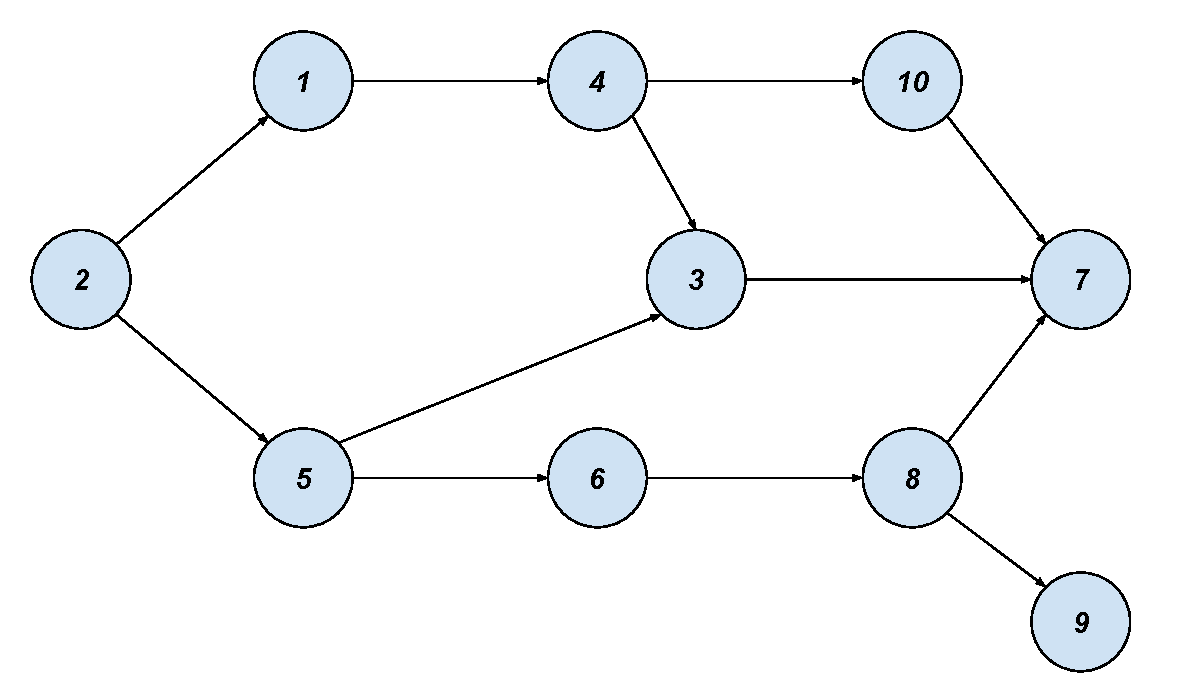
\includegraphics{graphs/floyd_warshall.pdf}
\end{figure}

$\mathfrak{D}_{ij}$ è l'insieme di tutti i cammini tra $i$ e $j$. \\
$\mathfrak{D}_{27} = \{\,<2,1,4,10,7>,\,<2,1,4,3,7>,\, <2,5,3,7>,\, <2,5,6,8,7>\}$

$\mathfrak{C}_{27}^{(1)} = \emptyset$ \\
$\mathfrak{C}_{27}^{(2)} = \emptyset$ \\
$\mathfrak{C}_{27}^{(3)} = \emptyset$ \\
$\mathfrak{C}_{27}^{(4)} = \{<2,1,4,3,7>\}$ (Cammino minimo e unico)\\
$\mathfrak{C}_{27}^{(5)} = \{<2,1,4,3,7>,\, <2,5,3,7>\}$ \\
Quindi $\mathfrak{C}_{ij}^{(n)} = \mathfrak{D}$ \\

\paragraph{Codice}

\lstinputlisting{code/floyd_warshall.txt}
Complessità : $\Theta(n^3)$

\[
W = D^0 =
 \begin{pmatrix}
  0 & 3 & 8 & \infty & -4 \\
  \infty & 0 & \infty & 1 & 7 \\
  \infty & 4 & 0 & \infty & \infty \\
  2 & \infty & -5 & 0 & \infty \\
  \infty & \infty & \infty & 6 & 0
 \end{pmatrix}
\]

\[
D^1 =
 \begin{pmatrix}
  0 & 3 & 8 & \infty & -4 \\
  \infty & 0 & \infty & 1 & 7 \\
  \infty & 4 & 0 & \infty & \infty \\
  2 & 5 & -5 & 0 & -2 \\
  \infty & \infty & \infty & 6 & 0
 \end{pmatrix}
\]

\[
D^2 =
 \begin{pmatrix}
  0 & 3 & 8 & 4 & -4 \\
  \infty & 0 & \infty & 1 & 7 \\
  \infty & 4 & 0 & 5 & 11 \\
  2 & 5 & -5 & 0 & -2 \\
  \infty & \infty & \infty & 6 & 0
 \end{pmatrix}
\]

\paragraph{Osservazioni}

\subparagraph{Osservazione A}

Se non ci sono cicli negativi, allora $\forall k,i = 1\ldots n, d_{ii}^{(k)} = 0$, ovvero ci sono solo valori nulli sulla diagonale principale.

\subparagraph{Dimostrazione per induzione su k}

Se $k=0$: VERO \\
Se $k>0$:

\begin{equation}
d_{ii}^{(k)} = min( \underbrace{d_{ii}^{(k-1)}}_\text{nullo per ipotesi} ,  \underbrace{d_{ik}^{(k-1)} + d_{ki}^{(k-1)}}_\text{positivo o nullo} ) = 0
\end{equation}

L'equazione risulta nulla poichè il primo termine $d_{ii}^{(k-1)}$ è nullo per ipotesi.
Il secondo termine non può essere negativo in quanto non ho cicli negativi.

\subparagraph{Osservazione B}

$\forall k = 1\ldots n,i,j \in V$

\[
\begin{cases} d_{ik}^{(k)} = d_{ik}^{(k-1)} \mbox{ Stessa colonna} \\ d_{kj}^{(k)} = d_{kj}^{(k-1)} \mbox{ Stessa riga} \end{cases}
\]

\subparagraph{Dimostrazione}

\begin{equation}
d_{ik}^{(k)} = min(  \underbrace{ d_{ik}^{(k-1)} , d_{ik}^{(k-1)}  }_\text{uguali} + \underbrace{ d_{kk}^{(k-1)} }_\text{nullo} ) = d_{ik}^{(k-1)}
\end{equation}

La stessa dimostrazione può essere applicata alla seconda equazione.

\subparagraph{Altre osservazioni}
Abbiamo notato che in caso appaia il valore \infty in una riga o in una colonna evidenziata, il valore delle altre celle non cambierà.

\subparagraph{Ottimizzazione}

Grazie alle osservazioni notiamo che possiamo utilizzare una sola matrice da sovrascrivere senza la necessità di averne una per ogni ciclo di $k$.

\lstinputlisting{code/floyd_warshall_sm.txt}